\documentclass[10pt,conference]{IEEEtran}
\usepackage{booktabs}
\usepackage{tabularx}
\usepackage{tikz}
\usetikzlibrary{arrows.meta,positioning}
\usepackage{array}
\usepackage{url}
\usepackage{hyperref}
\usepackage{xcolor}
\usepackage[T1]{fontenc}
\usepackage{soul}
\sethlcolor{yellow}
\newcommand{\todo}[1]{\hl{TODO: #1}}
\def\BibTeX{{\rm B\kern-.05em{\sc i\kern-.025em b}\kern-.08em T\kern-.1667em\lower.7ex\hbox{E}\kern-.125emX}}

\begin{document}

\title{ARC: A Dataset of Per-Service Damage Caused by Automated Remediation Actions in Microservice Systems}

\author{\IEEEauthorblockN{Laksh Jain, Abhishek Kumar Singh, Yogesh Choudhary, Ramakrishna Kolikipogu}
\IEEEauthorblockA{Department of Information Technology\\
Chaitanya Bharathi Institute of Technology (Autonomous), Hyderabad, India\\
Corresponding author: elitelaksh7@gmail.com \;\; \todo{confirm affiliations, emails, author order with guide}}}

\maketitle

\begin{abstract}
When a microservice system breaks, an operator or an automated agent applies a repair such as a restart, a scale-up or a drain. The repair can hurt services that were healthy, but no public dataset records how much. We present ARC, a dataset of 2{,}075 controlled incidents on two open-source systems (Train Ticket and Online Boutique) in which one of six remediation actions is applied after a fault and the damage to every service is measured. Each episode keeps the raw telemetry (per-service time series, call-graph edges, exact request and latency counters, the load generator's own request log, Kubernetes events) for 60~s before and 180~s after the action, and a per-service label: the rise in the share of bad requests. We describe how the data was collected, the files and labels, six evaluation splits, and four validity tests of the labels on both systems (negative control, dose--response, two independent instruments, and damage following the call graph). We also state the known limits: about 21\% of episodes are already saturated before the action, and the damage label averages over 180~s. The data is under CC BY 4.0 and the code under MIT.
\end{abstract}

\begin{IEEEkeywords}
microservices, remediation, blast radius, fault injection, AIOps, dataset
\end{IEEEkeywords}

\section{Introduction}
Automated remediation tools decide whether to act mostly by how confident they are in a root cause. Little is known about what the chosen action does to the services around its target: a drain can starve its callers, a rollout restart can make a healthy neighbour slow. Public datasets for operations of microservice systems record faults and their root causes~\cite{rcaeval,fang}, or whether an agent's decision was correct~\cite{dai,microremed,r7}; none records, per service, how much worse each service becomes after the repair. That quantity is needed to train a model that predicts the damage of an action before it is applied, and to evaluate agents that claim to remediate ``safely''~\cite{guarded}.

This paper describes ARC, a dataset built to fill that gap. Its contributions are:
\begin{itemize}
\item \textbf{Data.} 2{,}075 campaign episodes (1{,}795 on Train Ticket~\cite{trainticket}, 280 on Online Boutique~\cite{boutique}) with six actions and eight fault types plus no-fault, 120 healthy calibration episodes, and about 5.8 million recorded user requests.
\item \textbf{Labels with a stated meaning.} A per-service damage value for every episode, recomputable from raw counters with three latency bars.
\item \textbf{Validity evidence.} Four tests of the labels on both systems, since there is no external ground truth to compare with (Section~\ref{sec:valid}).
\item \textbf{Splits and loader} for six evaluation protocols, and a datasheet~\cite{gebru} that lists known issues.
\end{itemize}
The paper is a data descriptor; it makes no claim about a prediction method beyond the baseline use in Section~\ref{sec:uses}.

\section{Data Collection}
\textbf{Systems.} Train Ticket has 20--25 Java services behind one gateway. Online Boutique has 11 services plus a Redis cache; 10 are labelled, and for three of them (ad, cart, shipping) labels are derived from the callers' edge counters because the service itself is not instrumented. Both run on one Kubernetes cluster (kind, v1.34) on a single workstation (Intel Core i9-13900, 20 cores, 32~GB RAM). Faults are injected with Chaos Mesh~\cite{chaosmesh}; traces and metrics come from OpenTelemetry into Prometheus at 5~s resolution, with cAdvisor and kube-state-metrics for resources.

\textbf{Load.} An open-loop load generator (Poisson arrivals, nine user flows on Train Ticket; the shop's flows on Boutique) keeps the offered load constant even when the system slows. Load is 4 or 8 requests/s (Boutique: 8). Between episodes the database is trimmed so the healthy baseline does not drift.

\textbf{Episode.} One episode is a controlled incident: a fault is injected, 60--300~s later one action is applied, and everything is recorded for 60~s before and 180~s after (labelling starts 5~s after the action). The actions are no-op (control), restart-pod, rollout-restart, scale-up, cpu-bump and drain. The faults are none (control), pod-kill, hung pod, network delay, packet loss, CPU squeeze, database delay, call-cut and load surge. Episodes run unattended from a pre-registered plan of blocks of seven (one fault condition, each action once, no-op twice), so the no-op controls the same fault in the same block.

\begin{figure}[t]
\centering
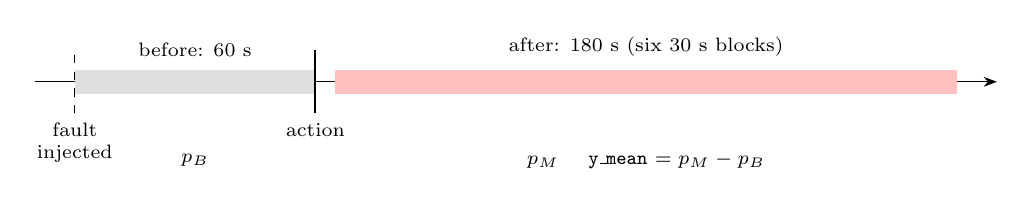
\begin{tikzpicture}[x=0.0105\columnwidth,y=1cm,>=Stealth,font=\scriptsize]
\draw[->] (0,0) -- (96,0);
\fill[gray!25] (4,-0.15) rectangle (28,0.15);
\fill[red!25] (30,-0.15) rectangle (92,0.15);
\draw[thick] (28,-0.4) -- (28,0.4);
\node[above] at (16,0.2) {before: 60 s};
\node[above] at (61,0.2) {after: 180 s (six 30 s blocks)};
\node[below] at (28,-0.4) {action};
\node[below,align=center] at (4,-0.4) {fault\\injected};
\node[below] at (29,-0.4) {};
\draw[dashed] (4,-0.4) -- (4,0.4);
\node[align=center] at (16,-1.0) {$p_B$};
\node[align=center] at (61,-1.0) {$p_M$ \quad \texttt{y\_mean} $=p_M-p_B$};
\end{tikzpicture}
\caption{One episode. The label is the rise in a service's share of bad requests.}
\label{fig:episode}
\end{figure}

\begin{table}[t]
\centering
\caption{Composition (campaign episodes). TT = Train Ticket.}
\label{tab:parts}
\footnotesize
\begin{tabularx}{\columnwidth}{@{}p{1.55cm}p{2.9cm}rX@{}}
\toprule
Part & System, load & Eps. & Faults \\
\midrule
batch1 & TT, 20 svc, 4 r/s & 701 & 5 types \\
wide1 & TT, 25 svc, 4 r/s & 500 & 5 types \\
wide1db & TT, 25 svc, 4 r/s & 126 & database delay \\
wide2 & TT, 25 svc, 8 r/s & 301 & 5 types \\
reptest & TT, 25 svc, 8 r/s & 20 & 4 recipes $\times$ 5 \\
held & TT, 25 svc, 8 r/s & 147 & call-cut, surge \\
boutique & Boutique, 8 r/s & 280 & 6 conditions \\
\midrule
Total & & 2{,}075 & \\
\bottomrule
\end{tabularx}
\end{table}

\begin{table}[t]
\centering
\caption{Episodes per action and per fault (both systems).}
\label{tab:counts}
\footnotesize
\begin{tabularx}{\columnwidth}{@{}XrXr@{}}
\toprule
Action & Eps. & Fault & Eps. \\
\midrule
no-op & 592 & packet loss & 537 \\
restart-pod & 299 & network delay & 504 \\
rollout-restart & 298 & none & 308 \\
drain & 298 & pod-kill & 308 \\
scale-up & 295 & hung pod & 154 \\
cpu-bump & 293 & CPU squeeze & 96 \\
 & & database delay & 63 \\
 & & call-cut & 63 \\
 & & load surge & 42 \\
\bottomrule
\end{tabularx}
\end{table}

\section{Data Description}
\textbf{Label.} For each service, the share of bad requests in the 60~s before the action ($p_B$) is compared with the share in the 180~s after it ($p_M$). A request is bad if it failed or exceeded a latency bar: a calibrated per-operation bar (healthy 99th percentile with a 100~ms floor, fitted on healthy calibration episodes), or a fixed 500~ms or 1~s bar. The label \texttt{y\_mean} is $p_M - p_B$ in points; \texttt{y\_peak} is the worst 30~s block. A service is scored only if it saw at least 30 requests in both windows. A verdict (harm, no\_harm, inconclusive, no\_data) and the time to recover are also given.

\textbf{Size.} Train Ticket: 37{,}790 labelled (episode, service) rows, 28{,}769 scored, 4{,}696{,}050 requests. Boutique: 2{,}800 rows, 2{,}726 scored, about 1.08 million requests. The raw archives are about 1~GB compressed.

\textbf{Files.} \texttt{episodes} (one row per episode: fault, action, load, saturation flag), \texttt{service\_labels}, \texttt{client\_flows}, \texttt{splits}, per-part raw archives (\texttt{services}, \texttt{edges}, \texttt{op\_counters}, \texttt{client}, \texttt{events}, \texttt{labels\_v2}, \texttt{meta}), a standard-library loader and a schema document. The six official splits are in-system, unseen system, unseen fault, held-out faults (call-cut, load surge), higher load and a noise ceiling from repeated identical incidents.

\textbf{Running example.} The loader uses only the standard library (pandas optional):
\begin{footnotesize}
\begin{verbatim}
import arc_data as arc
labels = arc.load_service_labels()
split  = arc.load_splits()
train  = [s["episode_id"] for s in split
          if s["unseen_system"] == "train"]
rows = [r for r in labels
        if r["episode_id"] in set(train)]
\end{verbatim}
\end{footnotesize}
\todo{extend loader and splits to cover the Boutique part before release}

\textbf{Privacy.} The users are a script with one test account; no personal data is involved. Host names and user paths were removed from the released JSON files.

\section{Validity of the Labels}\label{sec:valid}
No public benchmark scores repair damage per service, so the labels cannot be checked against someone else's answers. We tested them four ways on the campaign episodes of both systems (Table~\ref{tab:valid}).

\begin{table*}[t]
\centering
\caption{Validity tests of the damage labels (values in percentage points unless stated).}
\label{tab:valid}
\small
\begin{tabular}{@{}p{2.6cm}p{6.2cm}p{6.6cm}@{}}
\toprule
Test & Train Ticket (1{,}795 episodes) & Online Boutique (280 episodes) \\
\midrule
1. Negative control (no fault, no-op) & 3 of 1{,}288 scored rows harmed (0.2\%); healthy calibration 0 of 1{,}406 & 0 of 100 rows; healthy calibration 0 of 279 \\
2. Dose--response (bad-request share before the action, by fault level) & Loss: 7 of 7 targets positive (median Spearman 0.86); delay 7 of 7 (0.58); database delay weak ($\rho=0.21$) & Loss 5\%$\to$15\%: 0.4\%$\to$8.6\% ($p<10^{-10}$); delay 10$\to$25: 12.5\%$\to$24.9\% ($p=0.018$) \\
3. Two instruments (service counters vs.\ load-generator log) & Pearson 0.95, Spearman 0.86 (0.95 where an effect exists); counters read lower by 4.6 on average & Pearson 0.98, Spearman 0.89 (0.99 where an effect exists); drain 28.4 vs.\ 44.4 \\
4. Mechanism (excess over the same block's no-op, after a drain) & Direct callers +66.4, 2+ hops +68.3, callees +0.2, unrelated $-0.3$ & Direct callers +45.2, 2+ hops +10.7, callees 0.0, unrelated +2.3 (9\% harm verdicts) \\
\bottomrule
\end{tabular}
\end{table*}

Both systems give the same answers: labels stay at zero when nothing happens, rise with fault dose, agree with an independent instrument in rank, and appear where the call graph says they should. Two caveats come out of the tests. First, service-side counters read lower than the clients see when damage is large, so the labels are a conservative lower bound. Second, database-delay levels are not a severity scale (the dose--response relation is weak).

\section{Prior Use and Reuse}\label{sec:uses}
\textbf{Prior use.} We used the data to train and test a graph model that predicts the damage of an action from the state of every service, the call graph and the action. On the Train Ticket in-system protocol its mean absolute error is 1.98 points against 3.86 for a rule that uses the service's role in the call graph; it is also better on the unseen-system, unseen-fault and higher-load protocols, and ties the rule on held-out faults (7.57 vs.\ 7.51). The model and its evaluation are reported separately.

\textbf{Intended uses.} Training and testing models that predict per-service damage; ranking or gating candidate actions; blast-radius explanation; evaluating remediation agents on the damage they cause rather than only on whether they resolve the incident; studying how well damage predictions transfer between systems (the two systems share no service).
\textbf{Open questions.} Does a model trained on one system transfer to the other? Which inputs matter (call graph, action, role)? How early can damage be predicted from the first seconds of a fault? Are short bursts, which the 180~s label hides, predictable from the raw requests?

\section{Scope and Usage Notes}
The datasheet lists every known issue; the ones that change how the data should be used are these.
(1)~\textbf{Saturated episodes are flagged.} In 389 of 1{,}795 Train Ticket episodes and 59 of 280 Boutique episodes users were already at least 80\% bad before the action (\texttt{saturated\_before\_action}). Excluding them, or using the 1~s bar, gives a clean comparison of actions; including them is useful for studying overload. Hung-pod episodes are always saturated.
(2)~\textbf{Two systems, one machine.} Each system runs with one copy of each service on one workstation, with fault levels dosed on that machine; a level is a dose, not a severity scale. The number of replicas and the age of a fault are not recorded as inputs. Repeating the same incident gives a net effect within 12--27\% (coefficient of variation), which is the measurement noise of the benchmark.
(3)~\textbf{Time scale.} The label averages over 180~s, which suits actions with lasting effects (drain, restarts on Train Ticket, scale-up). Bursts of a few seconds, such as a Boutique restart of about 10~s, are in the raw requests and not in the label.
(4)~\textbf{Label meaning.} Labels measure what users see (the share of bad requests). Service-side counters read somewhat lower than the client log when damage is large, so the labels are a conservative lower bound. Three Boutique services are labelled from their callers' counters.
(5)~\textbf{Splits provided for known issues.} A first-half split of Train Ticket part wide2 avoids a drift in one flow; episodes affected by harness faults are listed in the release and excluded from the usable set.

\section{Availability}
The data is on Zenodo (archive with DOI \todo{reserve DOI; insert}) and Hugging Face (tables and loader), under CC BY 4.0. The testbed code, plans and label scripts are at \url{https://github.com/lakshjain7/arc-testbed} under MIT and are archived with the release (\todo{code release DOI}). Each part has a manifest and SHA-256 checksums; the datasheet, schema and a loader are included. Version 1.0 contains Train Ticket; version 1.1 adds Online Boutique and never edits v1.0 in place. \todo{review copy: private Zenodo link for reviewers}

\section{Related Datasets}
RCAEval~\cite{rcaeval} and the fault-propagation benchmark of Fang et al.~\cite{fang} provide telemetry for root-cause analysis; they have no repair action. MicroRemed~\cite{microremed} and the recovery-aware evaluation of Qi et al.~\cite{r7} test whether models propose a correct remediation; Dai et al.~\cite{dai} label each decision as resolved, partial or false remediation, which is the closest work but gives no per-service damage. AIOpsLab~\cite{aiopslab} and SREGym~\cite{sregym} offer live environments for agents. ARC adds the per-service consequence of the action, with raw data from which other labels can be recomputed.

\section{Conclusion}
ARC records what six repair actions do to every service of two microservice systems, with raw telemetry, labels that passed four validity tests, and a list of known limits. We hope it lets others train and compare models that predict the damage of a repair before it is applied.

\section*{Acknowledgment}
The authors thank the Research and Entrepreneurship (RNE) Lab at Chaitanya Bharathi Institute of Technology for providing the lab system on which all episodes were recorded.

\begin{thebibliography}{99}
\bibitem{dai} C. Dai et al., ``Safe Remediation as Risk-Constrained Intervention Decision in Microservice Systems,'' arXiv:2607.20005, 2026.
\bibitem{guarded} W. Cai et al., ``Can AI Remediate Backend Failures Safely? GuardedAct with Blast-Radius-Aware Sandboxing,'' arXiv:2609.11264, 2026.
\bibitem{microremed} L. Zhang et al., ``MicroRemed: Benchmarking LLMs in Microservices Remediation,'' arXiv:2511.01166, 2025.
\bibitem{r7} J. Qi et al., ``Can LLMs Really Recover Microservice Failures? A Recovery-Aware Evaluation of Diagnosis-to-Action Reasoning,'' arXiv:2607.04623, 2026.
\bibitem{aiopslab} Y. Chen et al., ``AIOpsLab: A Holistic Framework to Evaluate AI Agents for Enabling Autonomous Clouds,'' arXiv:2501.06706, 2025.
\bibitem{sregym} J. Clark et al., ``SREGym: A Live Benchmark for AI SRE Agents with High-Fidelity Failure Scenarios,'' arXiv:2605.07161, 2026.
\bibitem{rcaeval} L. Pham et al., ``RCAEval: A Benchmark for Root Cause Analysis of Microservice Systems with Telemetry Data,'' arXiv:2412.17015, 2024.
\bibitem{fang} A. Fang et al., ``Rethinking the Evaluation of Microservice RCA with a Fault Propagation-Aware Benchmark,'' FSE 2026. arXiv:2510.04711.
\bibitem{trainticket} X. Zhou et al., ``Fault Analysis and Debugging of Microservice Systems: Industrial Survey, Benchmark System, and Empirical Study,'' IEEE Trans. Softw. Eng., vol. 47, no. 2, pp. 243--260, 2021.
\bibitem{boutique} Google Cloud Platform, ``Online Boutique (microservices-demo),'' \url{https://github.com/GoogleCloudPlatform/microservices-demo}.
\bibitem{chaosmesh} Chaos Mesh, a cloud-native chaos engineering platform for Kubernetes, \url{https://chaos-mesh.org}.
\bibitem{gebru} T. Gebru et al., ``Datasheets for Datasets,'' Commun. ACM, vol. 64, no. 12, pp. 86--92, 2021.
\end{thebibliography}

\end{document}
